\documentclass[smaller]{beamer}
\usetheme[english]{Berlin}
\usepackage{ngerman}
\useoutertheme{infolines}
\beamertemplatenavigationsymbolsempty
\usepackage{pgfplots,tikz,subfigure}
\usepackage{amsmath,amsthm}
\usepackage{hyperref,graphics,graphicx,color,algorithm,algorithmic,enumerate}
\usepackage{mymacros,wrapfig,relsize}
\usepackage{pict2e}
\usepackage[utf8x]{inputenc}

\newcommand{\ri}{\mathrm{i}}
\newcommand{\T}{\mathsf{T}}
\renewcommand{\H}{\mathsf{H}}
\newcommand{\eps}{\varepsilon}
\newcommand{\To}{\rightarrow}
\newcommand{\sddots}{\scalebox{0.6}{$\ddots$}}
\usepackage[pdf]{pstricks}
\usepackage{sansmathfonts}
%\usepackage{arev}
%\renewcommand\familydefault{\sfdefault}

\DeclareMathOperator{\loc}{loc}
\DeclareMathOperator{\rank}{rank}
\DeclareMathOperator{\RE}{Re}
\DeclareMathOperator{\IM}{Im}
\DeclareMathOperator{\In}{In}
\DeclareMathOperator{\im}{im}
\DeclareMathOperator{\Gl}{Gl}
\DeclareMathOperator{\spa}{span}
\DeclareMathOperator{\ext}{{ext}}
\DeclareMathOperator{\ind}{ind}
\DeclareMathOperator{\normalrank}{normalrank}
\DeclareMathOperator{\essup}{ess\,sup}
\DeclareMathOperator{\vect}{vec}

\newcommand{\re}{\mathrm{e}}
\newcommand{\ddt}{\tfrac{\mathrm{d}}{\mathrm{d}t}}
\newcommand{\sys}[4]{\left[\begin{array}{c|c} #1 & #2 \\ \hline #3 & #4 \end{array}\right]}

\renewcommand{\tilde}{\widetilde}
\renewcommand{\hat}{\widehat}

\title[]{Optimierung f\"ur Studierende der Informatik}
\subtitle{-- 2. Vorlesung --}
\author[Matthias Voigt]{\textbf{Matthias Voigt$^{1,2}$}}
\institute[]{
\begin{columns}
%\begin{center}
\column{0.45\textwidth}{\centering {$^1$Universit\"at Hamburg \\ Fachbereich Mathematik \\ Hamburg \\ }}
\column{0.45\textwidth}{\centering {$^2$Technische Universit\"at Berlin \\ Institut f\"ur Mathematik \\ Berlin  \\}}
%\end{center}
\end{columns}
}
\date[]{Universit\"at Hamburg
\begin{columns}
\column{0.45\textwidth}{\centering 
\includegraphics[width = 1.2\textwidth]{uhh-logo.png}\\}
\end{columns}
}

\definecolor{tucgreen}{rgb}{0.0,0.5,0.27}
\definecolor{tucred}{rgb}{0.75,0,0}
\definecolor{tucorange}{rgb}{1.0,.5625,0}
\definecolor{mpired}{HTML}{990000}
\definecolor{mpigreen}{HTML}{5C871D}
\definecolor{mpiblue}{HTML}{006AA9}
\definecolor{mpibg1}{HTML}{5D8B8A}
\definecolor{mpibg2}{HTML}{BFDFDE}
\definecolor{mpibg3}{HTML}{A7C1C0}
\definecolor{mpibg4}{HTML}{7DA9A8}
\definecolor{mpigrey}{rgb}{0.9294,0.9294,0.8784}

\begin{document}

\maketitle

\begin{frame}
 \frametitle{Das Simplex-Verfahren -- der allgemeine Fall}
\textbf{LP-Problem in Standardform}.
\begin{align}
\begin{alignedat}{3}
\label{eq:2:12}
& \text{maximiere } & \sum\limits_{j=1}^{n}{c_jx_j} & & \\
& \rlap{unter den Nebenbedingungen} & & & \\
&& \sum\limits_{j=1}^{n}{a_{ij}x_j} &\ \leq &\ b_i \quad (i=1,\ldots, m),\ \\
&& x_j &\ \geq & 0 \quad (j=1,\ldots,n).\
\end{alignedat}
\end{align}

Wir führen wir zunächst \structure{Schlupfvariablen} $x_{n+1}, \ldots, x_{n+m}$ sowie eine Variable $z$ ein, die den Wert der \structure{Zielfunktion} angibt:
\begin{align}
\begin{alignedat}{3}
\label{eq:2:13}
x_{n+i} &\ := &\ b_i &\ - &\ \sum\limits_{j=1}^{n}{a_{ij}x_j} & \quad (i = 1,\ldots, m), \\
      z &\ := &\     &    &\ \sum\limits_{j=1}^{n}{c_jx_j}. &
\end{alignedat}
\end{align}
\end{frame}

\begin{frame}
 \frametitle{Das Simplexverfahren -- der allgemeine Fall}
 Unter Verwendung der Bezeichnungen aus \eqref{eq:2:13} kann man das LP-Problem \eqref{eq:2:12} auch wie folgt schreiben:
\begin{align}
\label{eq:2:12'}
%\tag{\ref*{eq:2:12}'}
\begin{alignedat}{3}
& \text{maximiere $z$} & & & \\
& \rlap{unter den Nebenbedingungen} & & & \\
&& x_1,\ldots,x_{n+m} &\ \geq &\ 0.
\end{alignedat}
\end{align}
Die folgende häufig verwendete Möglichkeit, das LP-Problem \eqref{eq:2:12} zu formulieren, ergibt sich direkt aus der Definition der Schlupfvariablen:
\begin{align}
\label{eq:2:12''}
%\tag{\ref*{eq:2:12}''}
\begin{alignedat}{4}
& \text{maximiere } & \sum\limits_{j=1}^{n}{c_jx_j} & & & & \\
& \rlap{unter den Nebenbedingungen} & & & & & \\
&& \sum\limits_{j=1}^{n}{a_{ij}x_j} &\ + &\ x_{n+i} &\ = &\ b_i & \quad (i=1,\ldots,m),\ \\
&& & & x_j &\ \geq &\ 0 & \quad (j=1,\ldots,n+m).\
\end{alignedat}
\end{align}
\end{frame}

\begin{frame}
 \frametitle{Lineare Gleichungssysteme}
 Im Verlauf des Simplexverfahrens ersetzt man in jeder Iteration eine zulässige Lösung $x_1, \ldots, x_{n+m}$ von \eqref{eq:2:12''} durch eine zulässige Lösung $\overline{x}_1, \ldots, \overline{x}_{n+m}$; dabei strebt man an, dass die neue Lösung besser als die alte ist, d.h., man möchte erhalten, dass
\[
\sum\limits_{j=1}^{n}{c_j\overline{x}_j} > \sum\limits_{j=1}^{n}{c_jx_j}
\]

gilt. In unserem obigen Beispiel wurde dies in jeder Iteration erreicht; \alert{wir werden jedoch (später) noch sehen, dass es auch nötig sein kann, Iterationen zuzulassen, in denen $\sum\limits_{j=1}^{n}{c_j\overline{x}_j} = \sum\limits_{j=1}^{n}{c_jx_j}$ gilt}.

In unserem obigen Beispiel haben wir gesehen, dass in jeder Iteration nicht nur eine zulässige Lösung $x_1, \ldots, x_{n+m}$ ermittelt wird, sondern dass in jeder Iteration auch ein lineares Gleichungssystem mit $m+1$ Gleichungen vorkommt. In unserem Beispiel 
hatten diese eine \structure{besondere Form}: Links traten immer drei der Variablen $x_1,\ldots,x_6$ auf sowie (in der letzten Zeile) $z$, während rechts immer nur die drei übrigen der Variablen $x_1, \ldots, x_6$ vorkamen. Außerdem waren die drei \structure{Gleichungssysteme \"aquivalent}, besitzen also dieselbe Lösungsmenge. 
\end{frame}

\begin{frame}
 \frametitle{Erinnerung: 3 Gleichungssysteme}
 \begin{align}
\begin{alignedat}{5}
\label{eq:2:3}
x_4 &\ = &\  5 &\ - &\ 2x_1 &\ - &\ 3x_2 &\ - &\  x_3,\ \\
x_5 &\ = &\ 11 &\ - &\ 4x_1 &\ - &\  x_2 &\ - &\ 2x_3,\ \\
x_6 &\ = &\  8 &\ - &\ 3x_1 &\ - &\ 4x_2 &\ - &\ 2x_3,\ \\
z   &\ = &     &    &\ 5x_1 &\ + &\ 4x_2 &\ + &\ 3x_3.\
\end{alignedat}
\end{align}
\begin{align}
\begin{alignedat}{5}
\label{eq:2:8}
x_1 &\ = &\  \tfrac{5}{2} &\ - &\ \tfrac{3}{2}x_2 &\ - &\ \tfrac{1}{2}x_3 &\ - &\ \tfrac{1}{2}x_4,\ \\
x_5 &\ = &\            1 &\ + &\           5x_2 &    &                 &\ + &\           2x_4,\ \\
x_6 &\ = &\  \tfrac{1}{2} &\ + &\ \tfrac{1}{2}x_2 &\ - &\ \tfrac{1}{2}x_3 &\ + &\ \tfrac{3}{2}x_4,\ \\
z   &\ = &\ \tfrac{25}{2} &\ - &\ \tfrac{7}{2}x_2 &\ + &\ \tfrac{1}{2}x_3 &\ - &\ \tfrac{5}{2}x_4.\
\end{alignedat}
\end{align}
\begin{align}
\begin{alignedat}{5}
\label{eq:2:10}
x_3 &\ = &\  1 &\ + &\  x_2 &\ + &\ 3x_4 &\ - &\ 2x_6,\ \\
x_1 &\ = &\  2 &\ - &\ 2x_2 &\ - &\ 2x_4 &\ + &\  x_6,\ \\
x_5 &\ = &\  1 &\ + &\ 5x_2 &\ + &\ 2x_4, &    &        \\
z   &\ = &\ 13 &\ - &\ 3x_2 &\ - &\  x_4 &\ - &\  x_6.\
\end{alignedat}
\end{align}
\end{frame}

\begin{frame}
 \frametitle{Tableaus, Basis- und Nichtbasisvariablen}
 Für Gleichungssysteme wie \eqref{eq:2:3}, \eqref{eq:2:8} und \eqref{eq:2:10} gibt es \textbf{unterschiedliche Bezeichnungen}:
\begin{itemize}
\item Chvátal benutzt beispielsweise die Bezeichnung \structure{dictionary};
\item im Buch von Cormen et al. wird die Bezeichnung \structure{Schlupfform} benutzt;
\item im Buch von Matou\v{s}ek und Gärtner werden derartige Gleichungssysteme \structure{Tableaus} genannt.
\end{itemize}

Wir verwenden den Begriff \structure{Tableau}. Diejenigen Variablen $x_j$, die in einem Tableau auf der linken Seite stehen, nennt man \structure{Basisvariablen}, die übrigen Variablen $x_j$ \structure{Nichtbasisvariablen}. Die Menge der Basisvariablen nennt man eine \structure{Basis}.
\begin{itemize}
\item Die Menge der zu den Basisvariablen $x_j$ gehörenden Indizes $j$ bezeichnen wir mit $B$;
\item  die Menge der Indizes $j$, die bei den Nichtbasisvariablen vorkommen, mit $N$.
\end{itemize}
Im Verlauf des Simplexalgorithmus ändern sich $B$ und $N$:
\begin{itemize}
\item Für das Tableau \eqref{eq:2:3} gilt $B = \{4, 5, 6\}$ und $N =
\{1, 2, 3\}$. 
\item Beim Übergang von \eqref{eq:2:3} zum Tableau \eqref{eq:2:8} verlässt $x_4$ die Basis und $x_1$ wird neu in die Basis aufgenommen; für das Tableau \eqref{eq:2:8} gilt also $B = \{1, 5, 6\}$ und $N = \{2, 3, 4\}$.
\end{itemize}
\end{frame}

\begin{frame}
 \frametitle{Weitere Begriffe}
 \begin{itemize}
 \item Einen Übergang von einem Tableau zum nächsten (wie von \eqref{eq:2:3} zu \eqref{eq:2:8}) nennt man \structure{Pivotschritt}, \structure{Basisaustauschschritt} oder \structure{Basistausch};
 \item diejenige Variable, die neu in die Basis aufgenommen wird, heißt \structure{Eingangsvariable};
 \item die Variable, die die Basis verlässt, heißt \structure{Ausgangsvariable}. Diejenige Zeile, in der vor dem Basistausch links die Ausgangsvariable steht, heißt \structure{Pivotzeile};
 \item diejenige Spalte, in der vor dem Basistausch die Eingangsvariable steht, heißt \structure{Pivotspalte}.
 \end{itemize}
 
\textbf{Beispiel:} Beim Übergang von \eqref{eq:2:8} zu \eqref{eq:2:10} ist $x_3$ die Eingangsvariable und $x_6$ ist die Ausgangsvariable. Die Zeile von \eqref{eq:2:8}, in der $x_6$ steht, ist die Pivotzeile dieses Basistauschs; die Spalte von \eqref{eq:2:8}, in der $x_3$ steht, ist die Pivotspalte.
\end{frame}

\begin{frame}
 \frametitle{Zurück zum allgemeinen Fall}
 Wir kehren zurück zum allgemeinen Fall \eqref{eq:2:12}. Unter einem zu \eqref{eq:2:12} gehörigen \structure{Tableau} verstehen wir ein System von $m+1$ linearen Gleichungen mit den Variablen $x_1,\ldots,x_{n+m}$ und $z$ sowie mit den folgenden Eigenschaften:
\begin{enumerate}[1)]
\item Jede Lösung dieses Gleichungssystems ist eine Lösung von \eqref{eq:2:13}; und umgekehrt.
\item Die Gleichungen sind nach $m$ der Variablen $x_1,\ldots,x_{n+m}$ (genannt \structure{Basisvariablen}) und nach $z$ aufgelöst; die übrigen $n$ Variablen heißen \structure{Nichtbasisvariablen}. Jede der Basisvariablen $x_j$ sowie $z$ ist im Gleichungssystem als Summe aus einer Konstanten und einer Linearkombination der Nichtbasisvariablen dargestellt.
\end{enumerate}

Etwas vereinfacht kann man 2) auch so aussprechen: \alert{Jede Basisvariable $x_j$ sowie $z$ wird durch die Nichtbasisvariablen ausgedrückt}.
\end{frame}

\begin{frame}
 \frametitle{Zulässige Tableaus}
 Die Eigenschaften 1) und 2) definieren, was man unter einem \structure{Tableau} versteht. Die Tableaus \eqref{eq:2:3}, \eqref{eq:2:8} und \eqref{eq:2:10} besaßen darüber hinaus noch die folgende Eigenschaft:
\begin{enumerate}[3)]
\addtocounter{enumi}{2}
\item  Werden auf der rechten Seite alle Variablen gleich Null gesetzt, so erhält man eine zulässige Lösung. (Mit anderen Worten: Setzt man alle Nichtbasisvariablen gleich Null, so wird keine der Basisvariablen negativ.)
\end{enumerate}

Tableaus mit dieser zusätzlichen Eigenschaft werden \structure{zulässige Tableaus} genannt.
\end{frame}

\begin{frame}
 \frametitle{Zulässige Basislösungen}
 \alert{Jedes zulässige Tableau beschreibt also eine zulässige Lösung von \eqref{eq:2:12}, die man erhält, wenn man alle Nichtbasisvariablen gleich Null setzt}. Aber nicht jede zulässige Lösung entsteht auf diese Art aus einem zulässigen Tableau; beispielsweise ist
\[
x_1=1,\quad x_2=0,\quad x_3=1,\quad x_4=2,\quad x_5=5,\quad x_6=3
\]
eine zulässige Lösung des Beispiel-LP-Problems, die jedoch nicht von einem zulässigen Tableau auf die beschriebene Weise abstammt.\\
\vspace*{0.2cm}
Zulässige Lösungen, die durch ein Tableau beschrieben werden (d.h., die aus einem Tableau dadurch entstehen, dass man alle Nichtbasisvariablen auf Null setzt), heißen \structure{zulässige Basislösungen}.\\
\vspace*{.2cm}
\alert{Eine auffallende Eigenschaft des Simplexalgorithmus ist, dass er nur mit zulässigen Basislösungen arbeitet und alle anderen zulässigen Lösungen ignoriert}.
\end{frame}

\begin{frame}
 \frametitle{Ein zweites Beispiel}
 \textbf{LP-Problem:}
\begin{align*}
\begin{alignedat}{5}
& \text{maximiere } & 5x_1 &\ + &\ 5x_2 &\ + &\ 3x_3 & & \\
& \rlap{unter den Nebenbedingungen} & & & & & & & \\
&&  x_1 &\ + &\ 3x_2 &\ + &\  x_3 &\ \leq &\ 3,\ \\
&& -x_1 &\   &\      &\ + &\ 3x_3 &\ \leq &\ 2,\ \\
&& 2x_1 &\ - &\  x_2 &\ + &\ 2x_3 &\ \leq &\ 4,\ \\
&& 2x_1 &\ + &\ 3x_2 &\ - &\  x_3 &\ \leq &\ 2,\ \\
&& & & & & \llap{$x_1, x_2, x_3$} &\ \geq &\ 0.\
\end{alignedat}
\end{align*}
\end{frame}

\begin{frame}
 \frametitle{Zul\"assiges Starttableau}
 \textbf{Zulässiges Starttableau:}
\begin{align}
\begin{alignedat}{5}
\label{eq:2:c1}
x_4 &\ = &\ 3 &\ - &\  x_1 &\ - &\ 3x_2 &\ - &\  x_3,\ \\
x_5 &\ = &\ 2 &\ + &\  x_1 &\   &\      &\ - &\ 3x_3,\ \\
x_6 &\ = &\ 4 &\ - &\ 2x_1 &\ + &\  x_2 &\ - &\ 2x_3,\ \\
x_7 &\ = &\ 2 &\ - &\ 2x_1 &\ - &\ 3x_2 &\ + &\  x_3,\ \\ \cline{1-9}
  z &\ = &\   &\   &\ 5x_1 &\ + &\ 5x_2 &\ + &\ 3x_3.\
\end{alignedat}
\end{align}
F\"ur eine bessere \"Ubersichtlichkeit trennen wir die Gleichung f\"ur $z$ vom Rest des Tableaus durch eine Linie. \\
Das zul\"assige Starttableau beschreibt die zul\"assige L\"osung
\[
x_1 = 0,\quad
x_2 = 0,\quad
x_3 = 0,\quad
x_4 = 3,\quad
x_5 = 2,\quad
x_6 = 4,\quad
x_7 = 2.
\]
Diese müssen wir jedoch nicht explizit hinschreiben, da Sie implizit durch das Tableau gegeben ist.
\end{frame}

\begin{frame}
 \frametitle{1. Iteration}
 In der 1. Iteration wollen wir den Wert für $z$ erhöhen -- momentan  können wir $x_1$, $x_2$ oder $x_3$ erhöhen. In der Praxis erhöht man oft die Variable mit dem größten Koeffizienten in der Gleichung für $z$, im Beispiel $x_1$ oder $x_2$. Wir entscheiden uns für $x_1$.
 Für wachsendes $x_1$ werden $x_4$, $x_6$, and $x_7$ kleiner und keine dieser Variablen sollte negativ werden. Die Bedingung $x_7 \ge 0$ is am restriktivsten, nämlich $x_1 \le 1$. Wir setzen $x_1 = 1$ und erhalten $x_7=0$. Wir müssen nun $x_1$ und $x_7$ im Tableau tauschen:
 \begin{equation}
\label{eq:2:c2}
x_1 = 1 - \tfrac{3}{2}x_2 + \tfrac{1}{2}x_3 - \tfrac{1}{2}x_7.
\end{equation}
Einsetzen von \eqref{eq:2:c2} in die restlichen Gleichungen von \eqref{eq:2:c1} liefert
\begin{align}
\begin{alignedat}{5}
\label{eq:2:c3}
x_1 &\ = &\ 1 &\ - &\ \tfrac{3}{2}x_2 &\ + &\  \tfrac{1}{2}x_3 &\ - &\ \tfrac{1}{2}x_7,\ \\
x_4 &\ = &\ 2 &\ - &\ \tfrac{3}{2}x_2 &\ - &\  \tfrac{3}{2}x_3 &\ + &\ \tfrac{1}{2}x_7,\ \\
x_5 &\ = &\ 3 &\ - &\ \tfrac{3}{2}x_2 &\ - &\  \tfrac{5}{2}x_3 &\ - &\ \tfrac{1}{2}x_7,\ \\
x_6 &\ = &\ 2 &\ + &\           4x_2 &\ - &\            3x_3 &\ + &\            x_7,\ \\ \cline{1-9}
  z &\ = &\ 5 &\ - &\ \tfrac{5}{2}x_2 &\ + &\ \tfrac{11}{2}x_3 &\ - &\ \tfrac{5}{2}x_7.\
\end{alignedat}
\end{align}
\end{frame}

\begin{frame}
 \frametitle{Die 2. Iteration}
 In unserem Beispiel sollte die nächste Basisvariable $x_3$ sein. Dies ist die einzige Nichtbasisvariable \eqref{eq:2:c3} deren Koeffizient in der letzten Zeile positiv ist. Nun ist die Bedingung $x_6 \ge 0$ am restriktivsten und somit müssen wir $x_3$ mit $x_6$ tauschen:
\begin{align}
\begin{alignedat}{5}
\label{eq:2:c4}
x_3 &\ = &\ \tfrac{ 2}{3} &\ + &\ \tfrac{ 4}{3}x_2 &\ + &\ \tfrac{1}{3}x_7 &\ - &\ \tfrac{ 1}{3}x_6,\ \\
x_1 &\ = &\ \tfrac{ 4}{3} &\ - &\ \tfrac{ 5}{6}x_2 &\ - &\ \tfrac{1}{3}x_7 &\ - &\ \tfrac{ 1}{6}x_6,\ \\
x_4 &\ = &\            1 &\ - &\ \tfrac{ 7}{2}x_2 &\   &\                &\ + &\ \tfrac{ 1}{2}x_6,\ \\
x_5 &\ = &\ \tfrac{ 4}{3} &\ - &\ \tfrac{29}{6}x_2 &\ - &\ \tfrac{4}{3}x_7 &\ + &\ \tfrac{ 5}{6}x_6,\ \\ \cline{1-9}
  z &\ = &\ \tfrac{26}{3} &\ + &\ \tfrac{29}{6}x_2 &\ - &\ \tfrac{2}{3}x_7 &\ - &\ \tfrac{11}{6}x_6.\
\end{alignedat}
\end{align}
\end{frame}

\begin{frame}
 \frametitle{Die 3. Iteration}
 Hier ist die Eingangsvariable $x_2$ und die Ausgangsvariable $x_5$. Pivotierung ergibt das Tableau
\begin{align}
\begin{alignedat}{5}
\label{eq:2:c5}
x_2 &\ = &\ \tfrac{ 8}{29} &\ - &\ \tfrac{ 8}{29}x_7 &\ + &\ \tfrac{5}{29}x_6 &\ - &\ \tfrac{ 6}{29}x_5,\ \\
x_3 &\ = &\ \tfrac{30}{29} &\ - &\ \tfrac{ 1}{29}x_7 &\ - &\ \tfrac{3}{29}x_6 &\ - &\ \tfrac{ 8}{29}x_5,\ \\
x_1 &\ = &\ \tfrac{32}{29} &\ - &\ \tfrac{ 3}{29}x_7 &\ - &\ \tfrac{9}{29}x_6 &\ + &\ \tfrac{ 5}{29}x_5,\ \\
x_4 &\ = &\ \tfrac{ 1}{29} &\ + &\ \tfrac{28}{29}x_7 &\ - &\ \tfrac{3}{29}x_6 &\ + &\ \tfrac{21}{29}x_5,\ \\ \cline{1-9}
  z &\ = &\            10 &\ - &\             2x_7 &\ - &\             x_6 &\ - &\              x_5.
\end{alignedat}
\end{align}

Nun kann keine Nichtbasisvariable in die Basis aufgenommen werden ohne den Wert von $z$ zu verringern. Dieses Tableau beschreibt also eine optimale Lösung. Diese ist
\[
x_1 = \tfrac{32}{29}, \quad
x_2 = \tfrac{8}{29}, \quad
x_3 = \tfrac{30}{29}
\]
mit $z = 10$.
\end{frame}

\begin{frame}
 \frametitle{Einige Konventionen}
 Das Ergebnis einer Iteration ist immer ein neues Tableau. Am Ende jeder Iteration wird dieses Ergebnis -- das neue Tableau also -- übersichtlich hingeschrieben, wobei einige \alert{Konventionen} zu beachten sind, die wir im zweiten Beispiel kennengelernt haben:
\begin{enumerate}
\item Die $z$-Zeile wird \alert{unten} notiert und durch einen Strich abgetrennt.
\item Im neuen Tableau wird die Zeile mit der Eingangsvariablen immer \alert{oben} hingeschrieben.
\item Die Variable, die neu auf der rechten Seite auftaucht -- die Ausgangsvariable -- schließt immer \alert{rechts} an.
\item Außerdem ist es für die Übersichtlichkeit wichtig, dass im Tableau gleiche Variablen immer \alert{genau untereinander} geschrieben werden.
\end{enumerate}
\end{frame}

\begin{frame}
 \frametitle{Noch einige Sprechweisen}
 Im LP-Problem \eqref{eq:2:12} hatten wir es ursprünglich mit den Variablen $x_1,\ldots,x_n$ zu tun. Anschließend kamen sofort weitere Variablen $x_{n+1}, \ldots, x_{n+m}$ hinzu, die wir \structure{Schlupfvariablen} genannt haben. Um uns besser ausdrücken zu können, fehlt noch ein Name für die ursprünglichen Variablen $x_1,\ldots,x_n$: Es ist üblich, diese Variablen als \structure{Problemvariablen} oder \structure{Entscheidungsvariablen} zu bezeichnen.
\end{frame}


\begin{frame}
\frametitle{Schwierigkeiten und Hindernisse und wie man sie überwindet}
\alert{Die Beispiele des letzten Kapitels waren absichtlich so gewählt, dass alles glatt ging.} Es kann in anderen Beispielen jedoch so sein, dass Schwierigkeiten auftreten. Wir wollen nun die Simplexmethode genau analysieren, die wichtigsten Details unter die Lupe zu nehmen und Hindernisse aus dem Weg räumen.

Schwierigkeiten könnte es in allen Phasen des Verfahrens geben:
\begin{enumerate}[1)]
\item Initialisierung,
\item Iteration,
\item Terminierung. 
\end{enumerate}
\end{frame}

\begin{frame}
  \frametitle{Probleme bei der Initialisierung}
  \begin{itemize}
  \item Unsere bisherigen Beispiele waren so gewählt, dass es niemals schwierig war, ein geeignetes Starttableau zu finden. \alert{Wir werden jedoch sehen, dass es nicht in jedem Fall so leicht ist, sich ein geeignetes Starttableau zu verschaffen}. 
  \item Außerdem könnte es sein, dass es gar kein zulässiges Starttableau gibt, da das vorliegende LP-Problem unlösbar ist. \alert{Frage: Wie findet man heraus, ob ein unlösbares LP-Problem vorliegt?}
  \end{itemize}
\end{frame}

\begin{frame}
 \frametitle{Probleme mit der Iteration}
 Eine der Fragen, die sich hier stellen: Was macht man, wenn im aktuellen Tableau keine geeignete Eingangs- oder Ausgangsvariable zu finden ist? Als Antwort wird sich ergeben, dass man nichts mehr tun braucht:
 \begin{itemize}
 \item Falls keine geeignete Eingangsvariable existiert, so ist die vorliegende Lösung \alert{optimal};
 \item falls eine geeignete Eingangsvariable gefunden werden kann, aber keine dazugehörige Ausgangsvariable existiert, so ist man ebenfalls fertig, da das Problem in diesem Fall \alert{unbeschränkt} ist.
 \end{itemize}
\end{frame}

\begin{frame}
 \frametitle{Probleme mit der Terminierung}
 Könnte das Verfahren in eine unendliche Schleife geraten? \\ \vspace*{0.2cm}
 \textbf{Antwort}: Ja, aber es handelt sich eher um eine theoretische Möglichkeit, die außerdem erfolgreich bekämpft werden kann.
\end{frame}

\begin{frame}
 \frametitle{Initialisierung (Vorbemerkung)}
 Ist das LP-Problem
\begin{align}
\begin{alignedat}{4}
\label{eq:3:1}
& \text{maximiere } & \sum\limits_{j=1}^{n}{c_jx_j} & & & \\
& \rlap{unter den Nebenbedingungen} & & & & \\
&& \sum\limits_{j=1}^{n}{a_{ij}x_j} &\ \leq &\ b_i & \quad (i=1,\ldots,m), \\
&& x_j &\ \geq &\ 0 & \quad (j=1,\ldots,n)\
\end{alignedat}
\end{align}
zu lösen, so haben wir bisher immer das Starttableau dadurch erhalten, dass wir die Formeln für die Schlupfvariablen hingeschrieben haben (zusammen mit $z$):
\end{frame}

\begin{frame}
 \frametitle{Initialisierung (Vorbemerkung)}
 \begin{align*}
\begin{alignedat}{3}
x_{n+1} &\ = &\ b_1 &\ - &\ \sum\limits_{j=1}^{n}{a_{1j}x_j}\ \\[-3mm]
 &\ \ \ \vdots & & & \\[-2mm]
x_{n+m} &\ = &\ b_m &\ - &\ \sum\limits_{j=1}^{n}{a_{mj}x_j}\ \\ \cline{1-5}
z &\ = &\ & & \sum\limits_{j=1}^{n}{c_jx_j}.
\end{alignedat}
\end{align*}
Als dazugehörige Startlösung konnten wir bislang immer $x_1=...=x_n=0$, $x_{n+1}=b_1, \ldots, x_{n+m}=b_m$ wählen. Das führt aber nur dann zu einer zulässigen Lösung, wenn $b_i \geq 0\ (i=1,\ldots,m)$ gilt!

\alert{Wenn eines der $b_i$ negativ ist, so erhält man auf diese Art keine zulässige Lösung}. Wie man diese Schwierigkeit bei der Initialisierung überwindet, soll jetzt noch nicht besprochen werden.
\end{frame}

\begin{frame}
 \frametitle{Iteration -- Wahl der Eingangsvariablen}
 Ist ein zulässiges Tableau gegeben, so hat man für die nächste Iteration zunächst eine Eingangsvariable auszuwählen.
\begin{itemize}
 \item Als Eingangsvariable wählt man, falls dies möglich ist, eine Nichtbasisvariable $x_j$, für die der Koeffizient $\overline{c}_j$ in der letzten Zeile (der $z$-Zeile) des aktuellen Tableaus positiv ist: $\overline{c}_j > 0$.
 \item Falls es kein derartiges $x_j$ gibt, falls also
\[
\overline{c}_j \leq 0
\]
für alle Koeffizienten $\overline{c}_j$ in der letzten Zeile des aktuellen Tableaus gilt, \alert{so liegt eine optimale Lösung vor}. \\
\textbf{Genauer:} Die letzte Zeile des aktuellen Tableaus lautet
\[
z = z^* + \sum\limits_{j \in N}{\overline{c}_jx_j},
\]
Falls nun $\overline{c}_j \leq 0$ für alle $j \in N$ gilt, so führt jede zulässige Lösung zu einem Wert der Zielfunktion $z$, der höchstens $z^*$ beträgt, da wegen $x_j \ge 0$ gilt, daß $\sum\limits_{j \in N}{\overline{c}_jx_j} \leq 0$.
\end{itemize}
\end{frame}

\begin{frame}
 \frametitle{Iteration: Wahl der Ausgangsvariablen}
 Als Ausgangsvariable wählt man, falls dies möglich ist, eine Basisvariable $x_i$, für die die Bedingung $x_i \geq 0$ zu einer möglichst strengen oberen Schranke für die Eingangsvariable führt.\\
 \vspace*{0.2cm}
\alert{Falls kein geeigneter Kandidat hierfür zur Verfügung steht, so ist das Problem unbeschränkt}\index{unbeschränkt}. Wir er\-läu\-tern diesen Fall an einem \textbf{Beispiel:}
\begin{align*}
\begin{alignedat}{5}
x_2 &\ = &\ 5 &\ + &\ 2x_3 &\ - &\  x_4 &\ - &\ 3x_1,\ \\ 
x_5 &\ = &\ 7 &    &       &\ - &\ 3x_4 &\ - &\ 4x_1,\ \\ \cline{1-9}
z   &\ = &\ 5 &\ + &\  x_3 &\ - &\  x_4 &\ - &\  x_1.\
\end{alignedat}
\end{align*}
Hier ist die Eingangsvariable $x_3$, jedoch führt weder die Bedingung $x_2 \geq 0$ noch die Bedingung $x_5 \geq 0$ zu einer oberen Schranke für die Eingangsvariable $x_3$. \\
\vspace*{0.2cm}
\textbf{Mit anderen Worten:} Setzen wir $x_1=x_4=0$, so können wir $x_3$ so groß machen, wie wir wünschen, die Bedingungen $x_2 \geq 0$ und $x_5 \geq 0$ werden dadurch nicht verletzt. Das Problem ist also unbeschränkt.
\end{frame}

\begin{frame}
\frametitle{Pivotierung}
Falls es mehrere geeignete Kandidaten für die Wahl der Ausgangsvariablen gibt, d.h., falls es mehrere Basisvariablen gibt, die zur selben möglichst strengen oberen Schranke für die Eingangsvariable führen, so kann man eine dieser Variablen beliebig auswählen.

Hat man eine Eingangsvariable und eine Ausgangsvariable gewählt, so ist die Pivotierung immer möglich.
\end{frame}

\begin{frame}
 \frametitle{Entartung}
 Für die Wahl der Ausgangsvariable kann es mehrere Kandidaten geben. \\
 \vspace*{0.2cm}
 \textbf{Beispiel}:
\begin{align*}
\begin{alignedat}{5}
x_4 &\ = &\ 1 &\   &       &\   &\      &\ - &\ 2x_3,\ \\
x_5 &\ = &\ 3 &\ - &\ 2x_1 &\ + &\ 4x_2 &\ - &\ 6x_3,\ \\ 
x_6 &\ = &\ 2 &\ + &\  x_1 &\ - &\ 3x_2 &\ - &\ 4x_3,\ \\ \cline{1-9}
z   &\ = &    &\   &\ 2x_1 &\ - &\  x_2 &\ + &\ 8x_3.\
\end{alignedat}
\end{align*}
Wählen wir $x_3$ als Eingangsvariable, so beschränken alle drei Basisvariablen $x_4$, $x_5$ und $x_6$ den Zuwachs von $x_3$ auf $\frac{1}{2}$. Sowohl $x_4$, $x_5$ und $x_6$ kommen also als Ausgangsvariable infrage. Wir wählen $x_4$ und erhalten das neue Tableau:
\begin{align*}
\begin{alignedat}{5}
x_3 &\ = &\ 0.5 &\   &       &\   &\      &\ - &\ 0.5x_4,\ \\
x_5 &\ = &\     &\ - &\ 2x_1 &\ + &\ 4x_2 &\ + &\   3x_4,\ \\ 
x_6 &\ = &\     &\   &\  x_1 &\ - &\ 3x_2 &\ + &\   2x_4,\ \\ \cline{1-9}
z   &\ = &\   4 &\ + &\ 2x_1 &\ - &\  x_2 &\ - &\   4x_4.\
\end{alignedat}
\end{align*}
\end{frame}

\begin{frame}
 \frametitle{Entartung}
 \alert{Dieses Tableau unterscheidet sich von allen Tableaus, die bislang vorkamen} dadurch, dass für die dazugehörige zulässige Lösung gilt: Nicht nur die Nichtbasisvariablen $x_1$, $x_2$ und $x_4$ sind gleich Null, sondern es gibt auch Basisvariablen, die gleich Null sind. Die zugehörige Lösung lautet:
\[
x_1=0,\quad x_2=0,\quad x_3=0.5,\quad x_4=0,\quad x_5=0,\quad x_6=0.
\]

Eine zulässige Basislösung wird \structure{degeneriert} (oder \structure{entartet}) genannt, wenn eine oder mehrere Basisvariablen gleich Null sind.
\end{frame}

\begin{frame}
 \frametitle{Entartete Iterationen}
 In der nächsten Iteration ist $x_1$ die Eingangsvariable und $x_5$ ist die Ausgangsvariable. Wie üblich berechnen wir aus $x_3 \geq 0$, $x_5 \geq 0$ und $x_6 \geq 0$ den größtmöglichen Zuwachs für die Eingangsvariable $x_1$. Wir erhalten diesmal (im Unterschied zu allen früheren Fällen), dass kein positiver Zuwachs möglich ist, da sich aus $x_5 \geq 0$ (und $x_2=x_4=0$) ergibt, dass $x_1=0$ gilt. \\
\vspace*{0.2cm}
\textbf{Also:} 
\begin{itemize}
\item $x_1$ bleibt unverändert gleich Null; 
\item die übrigen Variablen $x_2$, $x_3$, $x_4$, $x_5$, $x_6$ und $z$ ändern sich ebenfalls nicht, 
\item nur das Tableau geht durch den Austausch von $x_1$ und $x_5$ über in
\begin{align*}
\begin{alignedat}{5}
x_1 &\ = &\     &\   &\ 2x_2 &\ + &\ 1.5x_4 &\ - &\ 0.5x_5,\ \\
x_3 &\ = &\ 0.5 &\   &\      &\ - &\ 0.5x_4, &\   &\         \\ 
x_6 &\ = &\     &\ - &\  x_2 &\ + &\ 3.5x_4 &\ - &\ 0.5x_5,\ \\ \cline{1-9}
z   &\ = &\   4 &\ + &\ 3x_2 &\ - &\    x_4 &\ - &\    x_5.\
\end{alignedat}
\end{align*}
\end{itemize}
\textbf{Definition:} Eine Iteration im Simplexverfahren heißt \structure{degeneriert} (oder \structure{entartet}), wenn sich die zulässige Basislösung nicht ändert. 
\end{frame}

\begin{frame}
 \frametitle{Entartete Iterationen}
 Unsere letzte Iteration war also degeneriert. In unserem Beispiel ist auch die nächste Iteration degeneriert, die übernächste jedoch nicht.\\
 \vspace*{0.2cm}
\alert{Auch in praktischen Anwendungen kommen degenerierte Iterationen vor (sogar häufig); typischerweise wird der Stillstand jedoch, wie in unserem Beispiel, nach einigen Schritten überwunden}.\\
\vspace*{0.2cm}
Entartung könnte aber auch -- zumindest in der Theorie -- dazu führen, dass sich das Verfahren im Kreis bewegt. Mit diesem Phänomen befassen wir uns im Folgenden; man spricht vom \structure{Kreisen} des Verfahrens.
\end{frame}

\begin{frame}
 \frametitle{Terminierung}
 Man kann -- wie wir gleich sehen werden -- Beispiele konstruieren, für die das Simplexverfahren in eine \alert{unendliche Schleife} gerät. Aus der Sicht der Praxis ist die allerdings kein Problem: In praktischen Anwendungen scheint dieses Phänomen aller Erfahrung nach niemals aufzutreten.\\
 \vspace*{0.2cm}
\textbf{Beispiel}. Unser Anfangstableau lautet
\begin{align*}
\begin{alignedat}{6}
x_5 &\ = &\     &\ - &\ 0.5x_1 &\ + &\ 5.5x_2 &\ + &\ 2.5x_3 &\ - &\  9x_4,\ \\
x_6 &\ = &\     &\ - &\ 0.5x_1 &\ + &\ 1.5x_2 &\ + &\ 0.5x_3 &\ - &\   x_4,\ \\
x_7 &\ = &\   1 &\ - &\    x_1, &\   &\        &\   &\        &\   &\        \\ \cline{1-11}
z   &\ = &\     &\   &\  10x_1 &\ - &\  57x_2 &\ - &\   9x_3 &\ - &\ 24x_4.\
\end{alignedat}
\end{align*}
Wir verwenden die folgenden (üblichen) \alert{Regeln}:
\begin{itemize}
\item Als Eingangsvariable wird immer eine Nichtbasisvariable mit einem möglichst hohen Koeffizienten in der letzten Zeile gewählt.
\item Falls es mehrere Basisvariablen gibt, die für das Verlassen der Basis infrage kommen, so wählen wir die Variable mit dem kleinsten Index.
\end{itemize}
\end{frame}

\begin{frame}
 \frametitle{Kreisen}
 In unserem Beispiel ergeben sich in den ersten sechs Iterationen die folgenden Tableaus:
 
 \textbf{Nach der ersten Iteration:}
\begin{align*}
\begin{alignedat}{6}
x_1 &\ = &\     &\   &\ 11x_2 &\ + &\  5x_3 &\ - &\  18x_4 &\ - &\  2x_5,\ \\
x_6 &\ = &\     &\ - &\  4x_2 &\ - &\  2x_3 &\ + &\   8x_4 &\ + &\   x_5,\ \\
x_7 &\ = &\   1 &\ - &\ 11x_2 &\ - &\  5x_3 &\ + &\  18x_4 &\ + &\  2x_5,\ \\ \cline{1-11}
z   &\ = &\     &\   &\ 53x_2 &\ + &\ 41x_3 &\ - &\ 204x_4 &\ - &\ 20x_5.\
\end{alignedat}
\end{align*}

\textbf{Nach der zweiten Iteration:}
\begin{align*}
\begin{alignedat}{6}
x_2 &\ = &\     &\ - &\  0.5x_3 &\ + &\  2x_4 &\ + &\ 0.25x_5 &\ - &\  0.25x_6,\ \\
x_1 &\ = &\     &\ - &\  0.5x_3 &\ + &\  4x_4 &\ + &\ 0.75x_5 &\ - &\  2.75x_6,\ \\
x_7 &\ = &\   1 &\ + &\  0.5x_3 &\ - &\  4x_4 &\ - &\ 0.75x_5 &\ - &\ 13.25x_6,\ \\ \cline{1-11}
z   &\ = &\     &\   &\ 14.5x_3 &\ - &\ 98x_4 &\ - &\ 6.75x_5 &\ - &\ 13.25x_6.\
\end{alignedat}
\end{align*}
\end{frame}

\begin{frame}
 \frametitle{Kreisen}
 \textbf{Nach der dritten Iteration:}
\begin{align*}
\begin{alignedat}{6}
x_3 &\ = &\     &\   &\  8x_4 &\ + &\ 1.5x_5 &\ - &\ 5.5x_6 &\ - &\  2x_1,\ \\
x_2 &\ = &\     &\ - &\  2x_4 &\ - &\ 0.5x_5 &\ + &\ 2.5x_6 &\ + &\   x_1,\ \\
x_7 &\ = &\   1 &\   &\       &\   &\        &\   &\        &\ - &\   x_1,\ \\ \cline{1-11}
z   &\ = &\     &\   &\ 18x_4 &\ + &\  15x_5 &\ - &\  93x_6 &\ - &\ 29x_1.\
\end{alignedat}
\end{align*}

\textbf{Nach der vierten Iteration:}
\begin{align*}
\begin{alignedat}{6}
x_4 &\ = &\     &\ - &\ 0.25x_5 &\ + &\ 1.25x_6 &\ + &\ 0.5x_1 &\ - &\ 0.5x_2,\ \\
x_3 &\ = &\     &\ - &\  0.5x_5 &\ + &\  4.5x_6 &\ + &\   2x_1 &\ - &\   4x_2,\ \\
x_7 &\ = &\   1 &\   &\         &\   &\         &\ - &\    x_1, &\   &\         \\ \cline{1-11}
z   &\ = &\     &\   &\ 10.5x_5 &\ - &\ 70.5x_6 &\ - &\  20x_1 &\ - &\   9x_2.\
\end{alignedat}
\end{align*}
\end{frame}

\begin{frame}
 \frametitle{Kreisen}
 \textbf{Nach der fünften Iteration:}
\begin{align*}
\begin{alignedat}{6}
x_5 &\ = &\     &\   &\  9x_6 &\ + &\   4x_1 &\ - &\   8x_2 &\ - &\   2x_3,\ \\
x_4 &\ = &\     &\ - &\   x_6 &\ - &\ 0.5x_1 &\ + &\ 1.5x_2 &\ + &\ 0.5x_3,\ \\
x_7 &\ = &\   1 &\   &\       &\ - &\    x_1, &\   &\        &\   &\         \\ \cline{1-11}
z   &\ = &\     &\   &\ 24x_6 &\ + &\  22x_1 &\ - &\  93x_2 &\ - &\  21x_3.\
\end{alignedat}
\end{align*}
\textbf{Nach der sechsten Iteration:}
\begin{align*}
\begin{alignedat}{6}
x_6 &\ = &\     &\ - &\ 0.5x_1 &\ + &\ 1.5x_2 &\ + &\ 0.5x_3 &\ - &\   x_4,\ \\
x_5 &\ = &\     &\ - &\ 0.5x_1 &\ + &\ 5.5x_2 &\ + &\ 2.5x_3 &\ - &\  9x_4,\ \\
x_7 &\ = &\   1 &\ - &\    x_1, &\   &\        &\   &\        &\   &\        \\ \cline{1-11}
z   &\ = &\     &\   &\  10x_1 &\ - &\  57x_2 &\ - &\   9x_3 &\ - &\ 24x_4.\
\end{alignedat}
\end{align*}
\end{frame}

\begin{frame}
 \frametitle{Kreisen}
 \alert{Wir sind also wieder dort, wo wir angefangen haben}. Dies führt zu folgender Definition.\\
 \vspace*{0.2cm}
\textbf{Definition:}
Wir sagen, dass \structure{das Simplexverfahren kreist}, falls ein und dasselbe Tableau in zwei verschiedenen Iterationen auftritt.\\
\vspace*{0.2cm}
Kreisen hängt immer mit degenerierten Iterationen zusammen: \alert{Sämtliche Iterationen, die dazu geführt haben, dass ein Tableau wiederholt vorkam, müssen degeneriert gewesen sein}.\\
\vspace*{0.2cm}
Es könnte also -- zumindest in der Theorie -- vorkommen, dass das Simplexverfahren nicht endet, da es im Sinne der obigen Definition kreist. Könnte es noch andere Gründe geben, weshalb das Simplexverfahren nicht terminiert? Die Antwort ist \alert{nein}: \\\vspace*{0.2cm}

\textbf{Satz:}
Falls das Simplexverfahren nicht terminiert, so kreist es.
\end{frame}

\begin{frame}
 \frametitle{Die Blandsche Regel}
 Aus Sicht der Theorie möchte man Kreisen natürlich völlig ausschließen. Dies ist in der Tat möglich: Es gibt verschiedene Möglichkeiten hierfür, von denen die  \structure{Blandsche Regel} die interessanteste ist:
 \begin{itemize}
 \item Bei der Verwendung der Blandschen Regel spielt die Größe der positiven Koeffizienten in der $z$-Zeile gar keine Rolle; \alert{man wählt unter den Variablen mit positivem Koeffizienten in der $z$-Zeile einfach die Variable $x_k$ mit dem kleinsten Index $k$.}
 \item Kommen entsprechend mehrere Basisvariablen als Ausgangsvariablen in Betracht, \alert{so wähle man unter diesen die Variable mit dem kleinsten Index.} (Man beachte: Nicht alle Basisvariablen kommen als Ausgangsvariablen in Betracht, da nur zulässige Tableaus entstehen dürfen.)
 \end{itemize}
 \textbf{Satz (Blandsche Regel):}
Gibt es mehrere Möglichkeiten für die Wahl der Eingangs- bzw. Ausgangsvariablen, so wähle man immer den Kandidaten $x_k$ mit dem kleinsten Index $k$. \\ \vspace*{0.2cm}
 \textbf{Satz:}
Bei Verwendung der Blandschen Regel terminiert das Simplexverfahren.
\end{frame}

\begin{frame}
 \frametitle{Das Zweiphasen-Simplexverfahren}
 Nach diesen Ausführungen kommen wir auf den Punkt Initialisierung zurück.
 Wir betrachten ein Problem in Standardform, wobei mindestens eine der rechten Seiten negativ ist:
\begin{align*}
\begin{alignedat}{4}
& \text{maximiere } & \sum\limits_{j=1}^{n}{c_jx_j} & & \\
& \rlap{unter den Nebenbedingungen} & & &\\
&& \sum\limits_{j=1}^{n}{a_{ij}x_j} & \leq &\ b_i & \quad (i=1,\ldots,m), \\
&& x_j &\ \geq &\ 0 & \quad(j=1,\ldots,n).
\end{alignedat}
\end{align*}
Um ein zulässiges Starttableau und damit auch eine zulässige Startlösung zu finden, betrachtet man das folgende LP-Problem, das \alert{Hilfsproblem} genannt wird:
\end{frame}

\begin{frame}
 \frametitle{Das Hilfsproblem}
 \begin{align*}
\begin{alignedat}{5}
& \text{minimiere $x_0$} & & & & & \\
& \rlap{unter den Nebenbedingungen} & & & & & \\
&& \sum\limits_{j=1}^{n}{a_{ij}x_j} &\ - &\ x_0 &\ \leq &\ b_i & \quad (i=1,\ldots,m), \\
&&                                  &    &\ x_j &\ \geq &\   0 & \quad(j=0,\ldots,n).
\end{alignedat}
\end{align*}

Eine zulässige Lösung des Hilfsproblems lässt sich leicht angeben: Man braucht nur die Variablen $x_1,\ldots,x_n$ gleich Null zu setzen und $x_0$ hinreichend groß zu wählen. \alert{Das Hilfsproblem besitzt also immer eine zulässige Lösung}. Außerdem erkennt man sofort, dass Folgendes gilt:\\ \vspace*{0.2cm}
\textbf{Feststellung 1:}
Das ursprüngliche Problem besitzt genau dann eine zulässige Lösung, wenn das Hilfsproblem eine zulässige Lösung mit $x_0=0$ besitzt bzw. (anders gesagt), wenn der optimale Wert des Hilfsproblems gleich Null ist.
\end{frame}

\begin{frame}
 \frametitle{Das Hilfsproblem}
 Genauer gilt, dass sich die zulässigen Lösungen des ursprünglichen Problems und die optimalen Lösungen des Hilfsproblems, für die $x_0=0$ gilt, auf eine sehr einfache Art entsprechen:
\begin{enumerate}[1)]
\item Ist $(x_1,\ldots,x_n)$ eine zulässige Lösung des ursprünglichen Problems, so erhält man eine optimale Lösung des Hilfsproblems, wenn man zusätzlich $x_0=0$ setzt.
\item \label{page:3:1} Ist umgekehrt $(x_0,\ldots,x_n)$ eine optimale Lösung des Hilfsproblems, für die $x_0=0$ gilt, so ist $(x_1,\ldots,x_n)$ eine zulässige Lösung des ursprünglichen Problems.
\end{enumerate}
Wir erläutern nun das weitere Vorgehen anhand des folgenden \textbf{Beispiels:}
\begin{align*}
\begin{alignedat}{5}
& \text{maximiere } & x_1 &\ - &\ x_2 &\ + &\ x_3 & & \\
& \rlap{unter den Nebenbedingungen} & & & & & & & \\
&& 2x_1 &\ - &\  x_2 &\ + &\ 2x_3 &\ \leq &\  4,\ \\ 
&& 2x_1 &\ - &\ 3x_2 &\ + &\  x_3 &\ \leq &\ -5,\ \\ 
&& -x_1 &\ + &\  x_2 &\ - &\ 2x_3 &\ \leq &\ -1,\ \\ 
&& & & & & \llap{$x_1,x_2,x_3$} &\ \geq &\ 0.\
\end{alignedat}
\end{align*}
\end{frame}

\begin{frame}
 \frametitle{Beispiel}
 Das dazugehörige \alert{Hilfsproblem} lautet, wenn es als \alert{Maximierungsproblem} geschrieben wird:
\begin{align*}
\begin{alignedat}{6}
& \text{maximiere $-x_0$} & & & & & & & & &\\
& \rlap{unter den Nebenbedingungen} & & & & & & & & & \\
&& 2x_1 &\ - &\  x_2 &\ + &\ 2x_3 &\ - &\ x_0 &\ \leq &\  4,\ \\ 
&& 2x_1 &\ - &\ 3x_2 &\ + &\  x_3 &\ - &\ x_0 &\ \leq &\ -5,\ \\ 
&& -x_1 &\ + &\  x_2 &\ - &\ 2x_3 &\ - &\ x_0 &\ \leq &\ -1,\ \\ 
&& & & & & & & \llap{$x_0,x_1,x_2,x_3$} &\ \geq &\ 0.\
\end{alignedat}
\end{align*}
Schreibt man die Formeln für die Schlupfvariablen $x_4$, $x_5$ und $x_6$ sowie für die Zielfunktion $w$ auf, so erhält man für das Hilfsproblem das folgende Tableau:
\begin{align*}
\begin{alignedat}{6}
x_4 &\ = &\  4 &\ - &\ 2x_1 &\ + &\  x_2 &\ - &\ 2x_3 &\ + &\ x_0,\ \\
x_5 &\ = &\ -5 &\ - &\ 2x_1 &\ + &\ 3x_2 &\ - &\  x_3 &\ + &\ x_0,\ \\
x_6 &\ = &\ -1 &\ + &\  x_1 &\ - &\  x_2 &\ + &\ 2x_3 &\ + &\ x_0,\ \\ \cline{1-11}
w   &\ = &\    &\   &\      &\   &\      &\   &\      &\ - &\ x_0.\
\end{alignedat}
\end{align*}
\end{frame}

\begin{frame}
 \frametitle{Beispiel}
 \alert{Dieses Tableau ist \textbf{kein} zulässiges Tableau, es kann jedoch durch eine einzige Pivotierung in ein zulässiges Tableau verwandelt werden}. Diese Pivotierung folgt jedoch einem etwas anderen Schema, als bislang gewohnt: Man wählt $x_0$ als Eingangsvariable, obwohl $x_0$ in der letzten Zeile des Tableaus mit einem negativen Koeffizienten auftritt. Wählt man zusätzlich $x_5$ als Ausgangsvariable, so erhält man das nunmehr zulässige Tableau:
\begin{align}
\begin{alignedat}{6}
\label{eq:3:8}
x_0 &\ = &\  5 &\ + &\ 2x_1 &\ - &\ 3x_2 &\ + &\  x_3 &\ + &\ x_5,\ \\
x_4 &\ = &\  9 &\   &\      &\ - &\ 2x_2 &\ - &\  x_3 &\ + &\ x_5,\ \\
x_6 &\ = &\  4 &\ + &\ 3x_1 &\ - &\ 4x_2 &\ + &\ 3x_3 &\ + &\ x_5,\ \\ \cline{1-11}
w   &\ = &\ -5 &\ - &\ 2x_1 &\ + &\ 3x_2 &\ - &\  x_3 &\ - &\ x_5.\
\end{alignedat}
\end{align}
\end{frame}

\begin{frame}
 \frametitle{Der allgemeine Fall}
 Im allgemeinen Fall geht alles ganz entsprechend, man schreibt zunächst das Hilfsproblem als Maximierungsproblem auf:
\begin{align*}
\begin{alignedat}{5}
& \text{maximiere $-x_0$} & & & & & & \\
& \rlap{unter den Nebenbedingungen} & & & & & & \\
&& \sum\limits_{j=1}^{n}{a_{ij}x_j} &\ - &\ x_0 &\ \leq &\ b_i & \quad (i=1,\ldots,m), \\
&&                                  &    &\ x_j &\ \geq &\   0 & \quad (j=0,\ldots,n).\
\end{alignedat}
\end{align*}

Aufschreiben der Formeln für die Schlupfvariablen $x_{n+1},\ldots,x_{n+m}$ und für die Zielfunktion $w$ führt zum folgenden (nicht zulässigen) Tableau für das Hilfsproblem:
\begin{align*}
\begin{alignedat}{6}
x_{n+i} &\ = &\  b_i - \sum\limits_{j=1}^{n}{a_{ij}x_j} &\ + &\ x_0\ &\ \quad (i=1,\ldots,m), \\ \cline{1-6}
     w  &\ = &\                                         &\ - &\ x_0. &
\end{alignedat}
\end{align*}
\end{frame}

\begin{frame}
 \frametitle{Pivotierung in ein zulässiges Tableau}
 \alert{Dieses Tableau kann durch eine einzige Pivotierung in ein zulässiges Tableau verwandelt werden}: Als Eingangsvariable wählt man $x_0$ und als Ausgangsvariable $x_{n+k}$ wählt man eine Variable mit negativem $b_k$, für die $|b_k|$ maximal ist. \\
\vspace*{0.2cm}
Wir fahren mit unserem \textbf{Beispiel} fort. Da wir mit dem Tableau (\ref{eq:3:8}) nun ein \alert{zulässiges} Tableau für unser Hilfsproblem vorliegen haben, können wir das Hilfsproblem wie gewohnt mit dem Simplexalgorithmus lösen. Als Starttableau dient dabei \eqref{eq:3:8}. Im ersten Iterationsschritt ist $x_2$ die Eingangs- und $x_6$ die Ausgangsvariable. Man erhält:
\begin{align*}
\begin{alignedat}{6}
x_2 &\ = &\  1 &\ + &\ 0.75x_1 &\ + &\ 0.75x_3 &\ + &\ 0.25x_5 &\ - &\ 0.25x_6,\ \\
x_0 &\ = &\  2 &\ - &\ 0.25x_1 &\ - &\ 1.25x_3 &\ + &\ 0.25x_5 &\ + &\ 0.75x_6,\ \\
x_4 &\ = &\  7 &\ - &\  1.5x_1 &\ - &\  2.5x_3 &\ + &\  0.5x_5 &\ + &\  0.5x_6,\ \\ \cline{1-11}
w   &\ = &\ -2 &\ + &\ 0.25x_1 &\ + &\ 1.25x_3 &\ - &\ 0.25x_5 &\ - &\ 0.75x_6.\
\end{alignedat}
\end{align*}\label{page:3:3}
\end{frame}

\begin{frame}
 \frametitle{Fortsetzung des Beispiels}
 Nach der zweiten Iteration (Eingangsvariable $x_3$ und Ausgangsvariable $x_0$) erhält man:
\begin{align}
\begin{alignedat}{6}
\label{eq:3:9}
x_3 &\ = &\ 1.6 &\ - &\ 0.2x_1 &\ + &\ 0.2x_5 &\ + &\ 0.6x_6 &\ - &\ 0.8x_0,\ \\
x_2 &\ = &\ 2.2 &\ + &\ 0.6x_1 &\ + &\ 0.4x_5 &\ + &\ 0.2x_6 &\ - &\ 0.6x_0,\ \\
x_4 &\ = &\   3 &\ - &\    x_1 &\   &\        &\ - &\    x_6 &\ + &\   2x_0,\ \\ \cline{1-11}
w   &\ = &\     &\   &\        &\   &\        &\   &\        &\ - &\    x_0.\
\end{alignedat}
\end{align}
 Das Tableau \eqref{eq:3:9} ist optimal. Als optimale Lösung des Hilfsproblems erhält man:
\[
x_0=0,\quad
x_1=0,\quad
x_2=2.2,\quad
x_3=1.6.
\]

Aufgrund von 2) von Folie \pageref{page:3:1} ergibt sich als zulässige Lösung für das ursprüngliche Problem:
\[
x_1=0,\quad
x_2=2.2,\quad
x_3=1.6.
\]
\end{frame}

\begin{frame}
 \frametitle{Nützliche Feststellung}
 Wir haben somit herausgefunden, dass das ursprüngliche Problem eine zulässige Lösung besitzt. Noch viel nützlicher ist jedoch die folgende Feststellung. \\
 \vspace*{0.2cm}
\textbf{Feststellung 2:}
Darüber hinaus kann das Tableau \eqref{eq:3:9} auf einfache Art in ein zulässiges Tableau für unser ursprüngliches Problem verwandelt werden \alert{(Starttableau für unser ursprüngliches Problem!)}.

Hier ist das zulässige Tableau für unser ursprüngliches Problem, das sich aus \eqref{eq:3:9} ergibt:
\begin{align}
\begin{alignedat}{5}
\label{eq:3:10}
x_3 &\ = &\  1.6 &\ - &\ 0.2x_1 &\ + &\ 0.2x_5 &\ + &\ 0.6x_6, \\
x_2 &\ = &\  2.2 &\ + &\ 0.6x_1 &\ + &\ 0.4x_5 &\ + &\ 0.2x_6, \\
x_4 &\ = &\    3 &\ - &\    x_1 &\   &\        &\ - &\    x_6, \\ \cline{1-9}
  z &\ = &\ -0.6 &\ + &\ 0.2x_1 &\ - &\ 0.2x_5 &\ + &\ 0.4x_6. 
\end{alignedat}
\end{align}
\end{frame}

\begin{frame}
 \frametitle{Starttableau für das ursprüngliche Problem}
 Die ersten drei Zeilen von \eqref{eq:3:10} sind aus \eqref{eq:3:9} dadurch entstanden, dass der letzte Summand (derjenige, in dem $x_0$ vorkommt) in jeder dieser Zeilen weggelassen wurde. Anders gesagt: Man betrachtet nur noch Lösungen von \eqref{eq:3:9}, für die $x_0=0$ gilt. Die letzte Zeile ergibt sich wie folgt: Für die ursprüngliche Zielfunktion $z$ gilt
\[
z = x_1 - x_2+x_3.
\]

Ersetzt man hierin $x_2$ und $x_3$ gemäß der ersten beiden Zeilen von \eqref{eq:3:10}, so erhält man die letzte Zeile von \eqref{eq:3:10}.
\end{frame}

\begin{frame}
 \frametitle{Die entscheidende Regel}
 Aufgrund von 1) und 2) auf Folie \pageref{page:3:1} erkennt man, dass die beschriebene Methode zu einem zulässigen Tableau für das ursprüngliche Problem führt, das dann als Starttableau dienen kann. \alert{Klarerweise funktioniert das alles aber nur, wenn es einem wie im Beispiel gelingt, $x_0$ aus der Basis \glqq rauszuschmeißen\grqq}.\\

Um dies zu erreichen, verfährt man bei der Lösung des Hilfsproblems nach der folgenden \textbf{Regel}:\\ \vspace*{0.2cm}

Gibt es nach erfolgter Wahl der Eingangsvariablen mehrere geeignete Kandidaten für die Wahl der Ausgangsvariablen und ist $x_0$ unter diesen Kandidaten, so entscheide man sich für $x_0$.\\ \vspace*{0.2cm}

Man beachte: Nachdem man (am Anfang) ein zulässiges Tableau hergestellt hat, löst man das Hilfsproblem wie gewohnt mit dem Simplexverfahren. Das bedeutet: \alert{Es dürfen nur noch zulässige Tableaus auftreten und nur wenn $x_0$ eine Basisvariable ist, die zu einer möglichst strengen Schranke für die Eingangsvariablen führt, kann man $x_0$ aus der Basis ausscheiden lassen.}
\end{frame}

\begin{frame}
\frametitle{Fall 1: Die Regel kommt zum Einsatz}
Verfährt man nach der obigen Regel, so erhält man unmittelbar im Anschluss an die Anwendung dieser Regel ein Tableau, in dem folgende Situation vorliegt: $x_0$ ist nicht mehr in der Basis, weshalb für die zu diesem Tableau dazugehörige zulässige Basislösung $x_0=0$ gilt. Folglich gilt dann auch
\[
w = -x_0 = 0.
\]

\alert{Gelingt es also, $x_0$ aus der Basis ausscheiden zu lassen, so erhält man eine zulässige Basislösung des Hilfsproblems, für die $x_0 = 0$ und folglich auch $w=0$ gilt}. Diese Lösung ist eine \alert{optimale} Lösung des Hilfsproblems, da die Zielfunktion $w =-x_0$ nicht größer als Null werden kann (wegen $x_0 \geq 0$). \alert{In diesem Fall hat man erreicht, was man wollte}: Aus dem Schlusstableau für das Hilfsproblem kann man -- wie beschrieben -- ein {Starttableau} für das ursprüngliche Problem gewinnen.
 
\end{frame}

\begin{frame}
 \frametitle{Fall 2: Die Regel kommt nicht zum Einsatz}
 Es bleibt der Fall zu betrachten, dass wir mit dem Hilfsproblem fertig sind, obwohl die obige Regel nicht zum Einsatz gekommen ist: \alert{Dann wäre das Hilfsproblem gelöst, aber $x_0$ wäre am Ende immer noch eine Basisvariable}. \\ \vspace*{0.2cm}

 \textbf{Behauptung}. Liegt dieser Fall vor, so gilt am Ende $w<0$. \\ \vspace*{0.2cm}
 
 Man beachte: Dass man bei der Lösung des Hilfsproblems am Schluss den optimalen Zielfunktionswert $w<0$ erhält, bedeutet, dass es nur Lösungen des Hilfsproblems mit $x_0>0$ gibt (wegen $w=-x_0$). Das heißt (vgl. Feststellung 1): \alert{Das ursprüngliche Problem besitzt keine zulässige Lösung.}
\end{frame}

\begin{frame}
 \frametitle{Das Zweiphasen-Simplexverfahren}
 Das beschriebene Verfahren ist unter dem Namen \structure{Zweiphasen-Simplexverfahren} bekannt:
\begin{itemize}
\item Liegt ein \alert{LP-Problem in Standardform} vor, so stellt man in der \alert{ersten Phase} zunächst das Hilfsproblem auf und löst es wie beschrieben; falls dies mit $w<0$ endet, so besitzt das ursprüngliche Problem keine zulässige Lösung; falls am Ende der ersten Phase $w=0$ gilt, so erhält man ein \alert{Starttableau für die zweiten Phase}.
\item In der \alert{zweiten Phase} löst man das ursprüngliche Problem.
\end{itemize}

Gilt $b_i \geq 0\ (i=1,\ldots,m)$, so entfällt die 1. Phase.
\end{frame}

\begin{frame}
 \frametitle{Fundamentalsatz der linearen Programmierung}
 \textbf{Satz (Fundamentalsatz der Linearen Programmierung):}
Für jedes LP-Problem $L$ in Standardform gilt genau eine der folgenden drei Aussagen:
\begin{enumerate}[1)]
\item $L$ besitzt eine optimale Lösung.
\item $L$ ist unlösbar.
\item $L$ ist unbeschränkt.
\end{enumerate}

\textbf{Beweis.} Die erste Phase des Zweiphasen-Simplexverfahrens führt entweder zu der Feststellung, dass $L$ unlösbar ist, oder man erhält ein Starttableau für die zweite Phase. In der zweiten Phase wird entweder festgestellt, dass das Problem unbeschränkt ist, oder man erhält eine optimale Lösung. \hfill $\Box$
\end{frame}

\begin{frame}
 \frametitle{Graphische Darstellung}
 \begin{center}
 \hspace*{-1.5cm}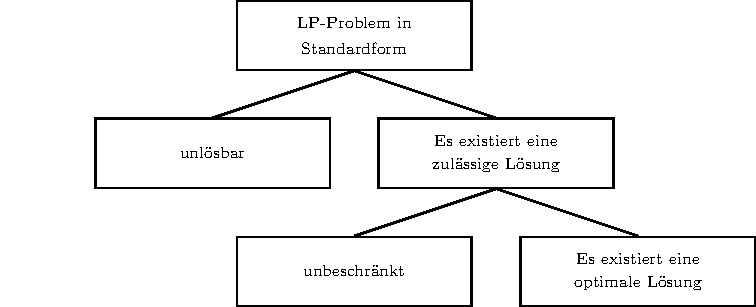
\includegraphics{fig5.pdf}
 \end{center}
\end{frame}


\end{document}
